\chapter{Data}
        In this chapter, we introduce the data used in this work and discuss methods by which we processed and engineered new features. 
        
         We used the Freddie Mac Single-Family dataset which contains approximately 95 million mortgages, with over 2 billion monthly observations covering approximately 60\% of all mortgages originated in the U.S. from January 1999 to January 2017. The loans are fully amortising 15, 20, and 30-year fixed-rate mortgages. The data itself is divided into origination records and performance records. We will refer to these separately, as 'Origination' features (described in Appendix \ref{appendix: table_american_loan_features_origination}), and 'Performance' features (described in Appendix \ref{appendix: table_american_loan_features_monthly}). A summary of key origination features and loan length can be seen in table \ref{4: summary_features}.
        
        
        \begin{center}
            \begin{table}[]
                \centering
                \begin{tabular}{|p{6cm}|p{1.75cm}|p{1.75cm}|p{1.75cm}|p{1.75cm}|}
                    \hline \textbf{Loan Feature} & \textbf{Mean} & \textbf{Median} & \textbf{Min} & \textbf{Max}  \\ \hline \hline
                    
                    Original Unpaid Balance (\$) & 191,114 & 148,388 & 9 & 5,400,000 \\ \hline
                    Interest Rate & 5.6 & 5.7 & 0 & 19.4 \\ \hline
                    Loan-To-Value Ratio & 75 & 78 & 0 & 203 \\ \hline
                    FICO Credit Score & 727 & 743.5 & 300 & 850 \\ \hline
                    Loan Length & 21.1 & 20 & 0 & 140 \\ \hline
                \end{tabular}
                \caption{Summary statistics for loan length and a subset of Origination features}
                \label{4: summary_features}
            \end{table}
        \end{center}
        
        
        % The monthly updates allow the corresponding labels to be determined, 'Good' if the mortgage was paid back in full and 'Bad' if it was not. 
        
    
    \section{Data Format} \label{data_format}
        The dataset is split into two sections, 'Origination' features and 'Performance' features. Individually, these records are separated into files and folders on a per quarterly basis. Each quarter contains the origination data for all mortgages that began during that period, as well as the corresponding performance updates over the lifetime of the mortgages. Each file is in CSV format, and range in size from 100MBs to 1.6GBs. 
    
    \section{Data Labelling} \label{data_labelling}
        
        % In order to model our problem, as discussed in \ref{chpt: Introduction}, we created multiple labels types. 

        % This allows us to train multiple networks where we optimise for different objective, which is especially important given the non-linear nature of the problem i.e. We do not only want to identify loans that pay back without default, we also want to considered fluctuations in repayment amounts (delinquency), and total amounts repaid given loan interest rates.
        
        A loan can be in status: Current, 30, 60, 90+ days delinquent, Foreclosed\footnote{It's is not uncommon for a vendor to move a mortgage into a default/foreclosed status to provoke repayment. After repayment, the loan transitions from default back to current.}, REO (Real-Estate Owned) or Fully Paid, which are defined in more detail in table \ref{appendix: table_american_loan_labels}. To determine a loan's status, we use the data columns; 'Delinquency Status', 'Zero Balance Code' and 'Repurchase Flag'. The exact rules we used can be seen in Appendix \ref{appendix: loan_state_rules}, along with the Zero Balance Code definitions in Appendix \ref{appendix: zero_balance_codes}.
        
        \begin{table}[H]
            \centering
                \begin{tabular}{|p{5cm}|p{9cm}|}
    
                    \hline \textbf{Loan Status} & \textbf{Description} \\ \hline \hline
                    Current (0)            & Loan is up to date on all outstanding payments, or within grace period. \\ \hline
                    30 days delinquent (1) & Loan has not been current for 30 to 60 days. \\ \hline
                    60 days delinquent (2) & Loan has not been current for 60 to 90 days. \\ \hline
                    90+ days delinquent (3) & Loan has not been current for 90+ days. \\ \hline
                    Foreclosed (4) & Loan has been foreclosed because payments have stopped. Property is being taken back by mortgage lender. \\ \hline
                    REO (Real-Estate Owned) (5)  & Loan has been foreclosed because payments have stopped. Property has been taken back by mortgage lender. \\ \hline
                    Fully Paid (6)  & Loan has been fully repaid, either at the expiration, or as a result of a prepayment. \\ \hline
                    \end{tabular}
                \caption{Loan Status Descriptions}
                \label{appendix: table_american_loan_labels}
        \end{table}

        
        \subsection{Label: Default or Fully Paid}  \label{labeling}
            To determine the binary 'Default' or 'Fully Paid' label, we identified the final status of each loan from the last performance update. There exist three possible final statuses, Foreclosed, REO (Real-Estate Owned) or Fully Paid. Once we have identified the final status of the loan, we reduce the status to either Fully Paid or Default. We classify loans in the Fully Paid status as Fully Paid, and loans in Foreclosed or REO status as Default. Finally, we reject all loans without a final terminating status. As many of the loans are still active, and therefore do not have a terminating status, this reduces the dataset to approximately a sixth of its original size. The class distribution between Default and Fully Paid loans can be seen in table \ref{table_class_dist}.  
            
            \begin{center}
                \begin{table}[]
                    \centering
                    \begin{tabular}{|p{9.0cm}|p{2.5cm}|p{2.5cm}|}
                        \hline \textbf{Metric} & \textbf{Default} & \textbf{Fully Paid} \\ \hline \hline
        
                        Total Number & 84,745 & 15,214,584 \\ \hline
                        Ratio & 0.006 & 0.994 \\ \hline
                    \end{tabular}
                    \caption{Class Distribution between Default and Fully Paid} \vspace{0.5cm}
                    \label{table_class_dist}
                \end{table}
            \end{center}
            
        % \subsection{Label: Delinquent matrix at time t}
        %     To determine the 'Delinquent matrix', we create forward look ahead state labels at time t for 18 consecutive months, as discussed in Section \ref{sec: Feature_Engineering}. We now have labels which map loan data at time t, to a loan state at t + 1-18 months, where a loan state can be seven possible categories: Current, 30, 60, 90+ days delinquent, Foreclosed, REO (Real-Estate Owned) or Fully Paid. This produces a 18 x 7 Delinquent matrix of possible states. 
        
        % \subsection{Label: Prepaid Ratio}
        %     To determine the 'Prepaid Ratio' label, we divide the Original Unpaid Balance by the length of the loan. A low 'Prepaid Ratio' represents a loan that has been paid back at a consistent rate over a long period of time. It is important to note that unlike the category labels discussed above, the 'Prepaid Ratio' label is a continuous values and will either require categorisation using set ranges, or a regression based approach.
        %     \unsure[inline]{Reword this bit maybe - "regression based approach"? }
        
    

    \section{Data Cleaning}\label{data_cleaning}
        There exists a small percentage of loans in the dataset with missing data values. Two possible reasons are either a reporting error by the original mortgage vendor or incomplete information provided by the borrower during the mortgage application. We, therefore, removed any entries in the origination data where the features FICO score, original balance, or original interest rate were missing. These features are required by a vendor when taking out the loan, and therefore we deduce that the absence of this data must be due to a reporting error. From the performance updates, we remove all loans which are missing the features Current Unpaid Balance, Delinquency Status, or Current Interest rate. 
        
        There exist additional features in the dataset that would not be required by all vendors at origination, for example, debt-to-income ratio. In these instances, we add a feature which indicates whether the data was missing or not (1 missing, 0 not missing). We then impute the missing value using the median. For features with categorical variables, we forgo the additional feature indicator and simply replace the value with a 'U' for Unknown. 
        
        After analysing the performance updates, we observed that many of the defined features are only relevant at the end of the mortgage, e.g. net sale proceeds, expenses, zero balance flag. We therefore removed all features from the performance updates that do not provide additional information during the active lifetime of the loan. We observed that a number of loans do not have a final state as a consequence of a reporting error. In these cases, they are removed. We also removed all loans that were ongoing, i.e. they still had an Unpaid balance in Q1 2017, and were not Foreclosed or REO. After this filtering process, we were left with approximately 15.3 million unique loans from which we had 326 million performance updates.
        
        For each categorical feature in the dataset, we defined a set of allowed values. For instances that contained values not defined in the set, we assigned a 'U' for Unknown. Similarly, for each numerical feature in the dataset, we defined an allowed value range. For instances that fell outside of the defined range, we added a feature indicating whether the data was missing or not (1 missing, 0 not missing), and impute the missing value using the median of the feature.
        

    \section{Feature Engineering} \label{sec: Feature_Engineering}
    
    
        \subsection{Origination Features}
        
            We observed that the origination feature set supplied by Freddy Mac (see appendix \ref{appendix: table_american_loan_features_origination}) contained a number of well researched and common mortgage indicators. For example, \cite{default_risk_2005} found that higher FICO scores resulted in higher prepayment rates. We found that lower FICO scores resulted in an increased likelihood of Default, with the opposite being true for higher scores. This is shown in density plot in figure \ref{fig:FICO_score}. 
            
            \begin{figure}[H]
                \centering
                \hspace*{-0.5cm}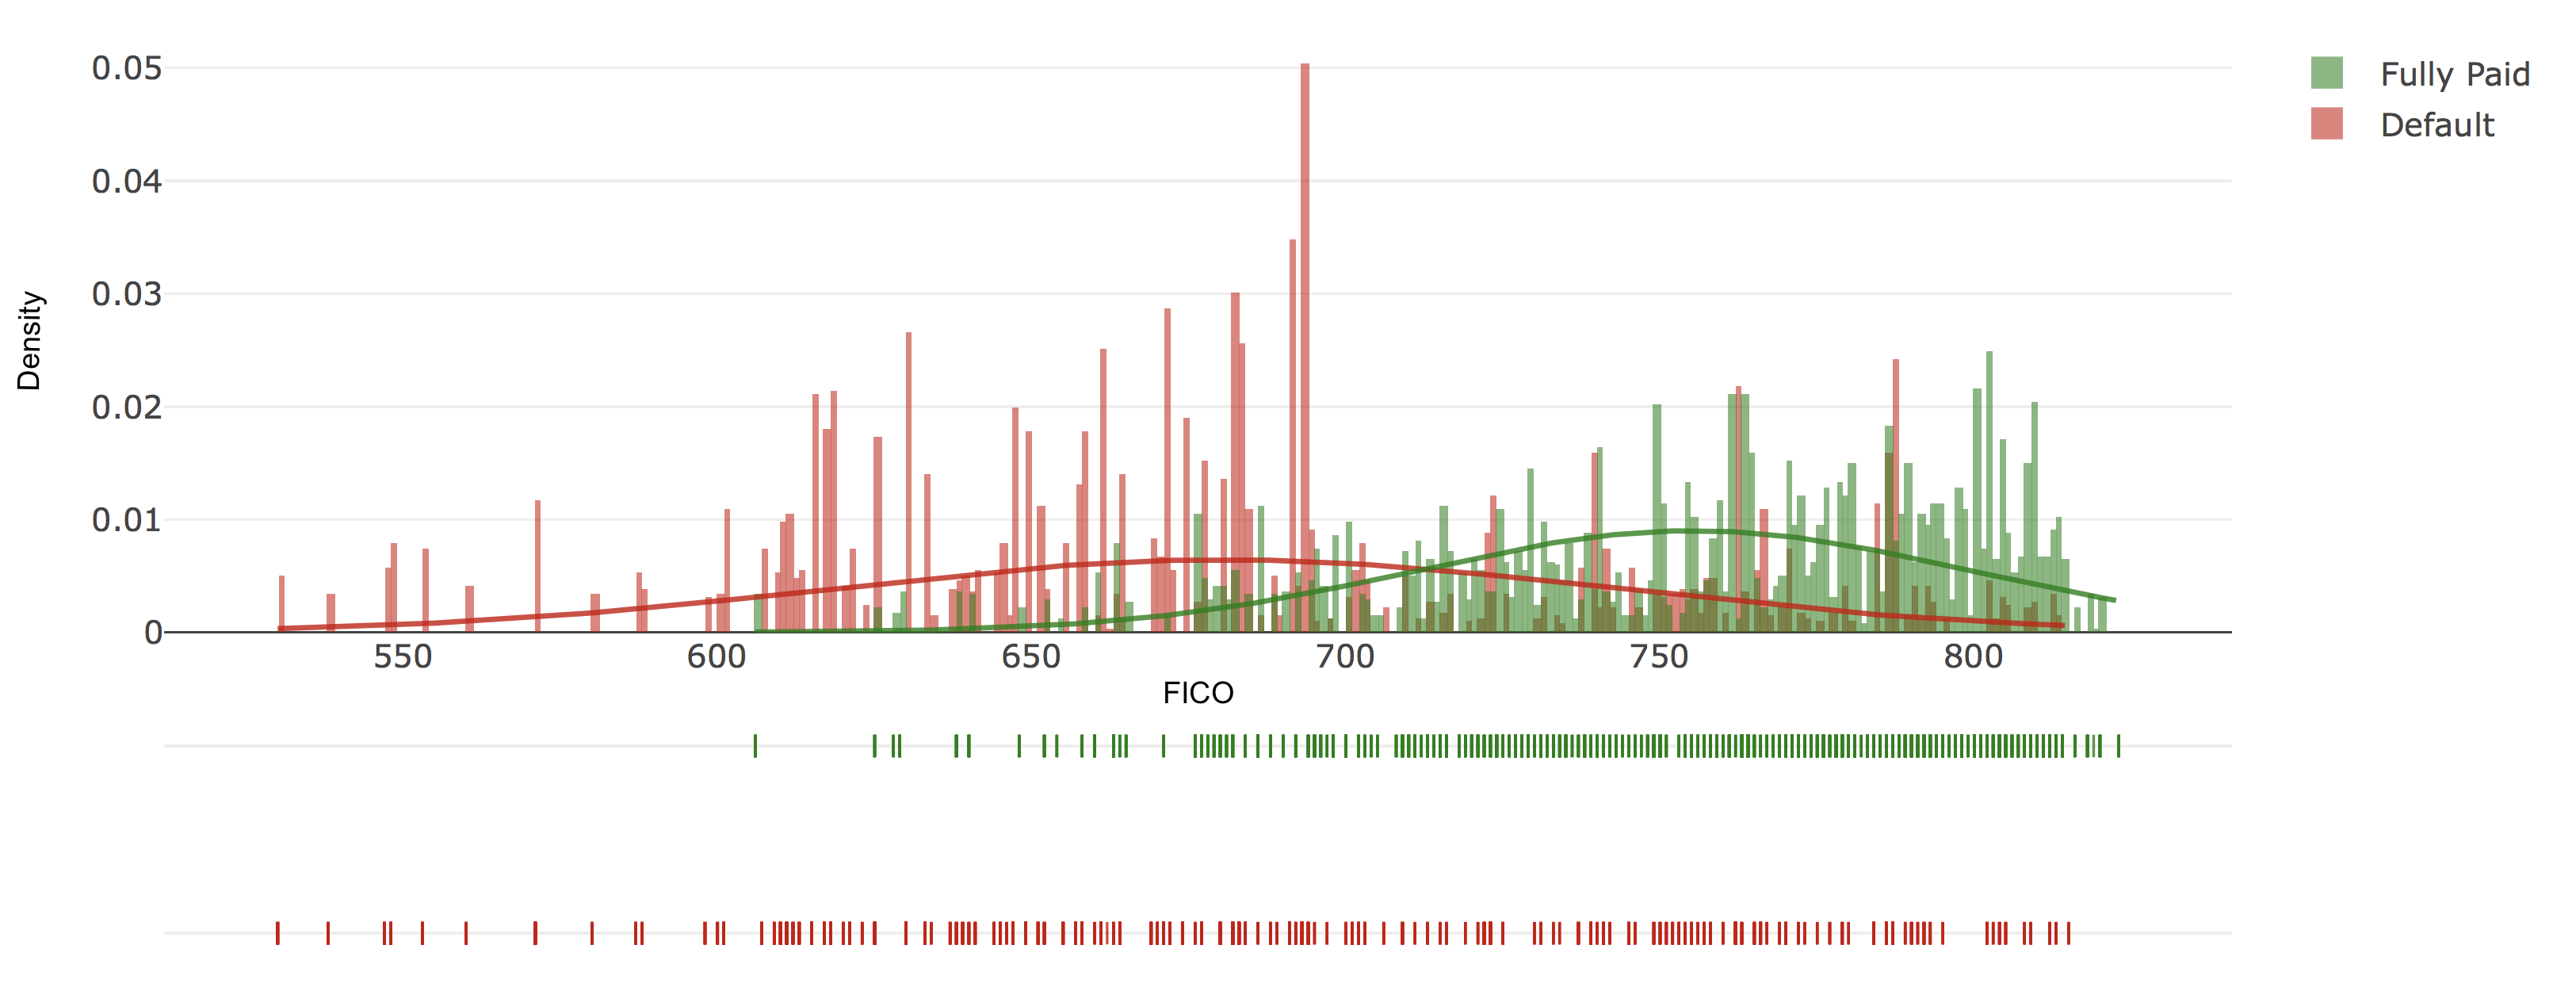
\includegraphics[width=1.1\textwidth]{Images/fico_dist.png}
                \caption{Density Plot with Normal Distribution and Rug plot - A comparison between Fully Paid and Default loans using the feature FICO Score}
                \label{fig:FICO_score}
            \end{figure}
            
            Another example is the feature Loan-to-Value (LTV) ratio. \cite{foreclosure_single_family_1998} found that higher Loan-to-Value ratios had a higher foreclosure probability. Our findings seem to support this observation. The density plot in figure \ref{fig:ltv} shows a small correlation between higher LTV ratios and the probability of default. 
            
            \begin{figure}[H]
                \centering
                \hspace*{-0.5cm}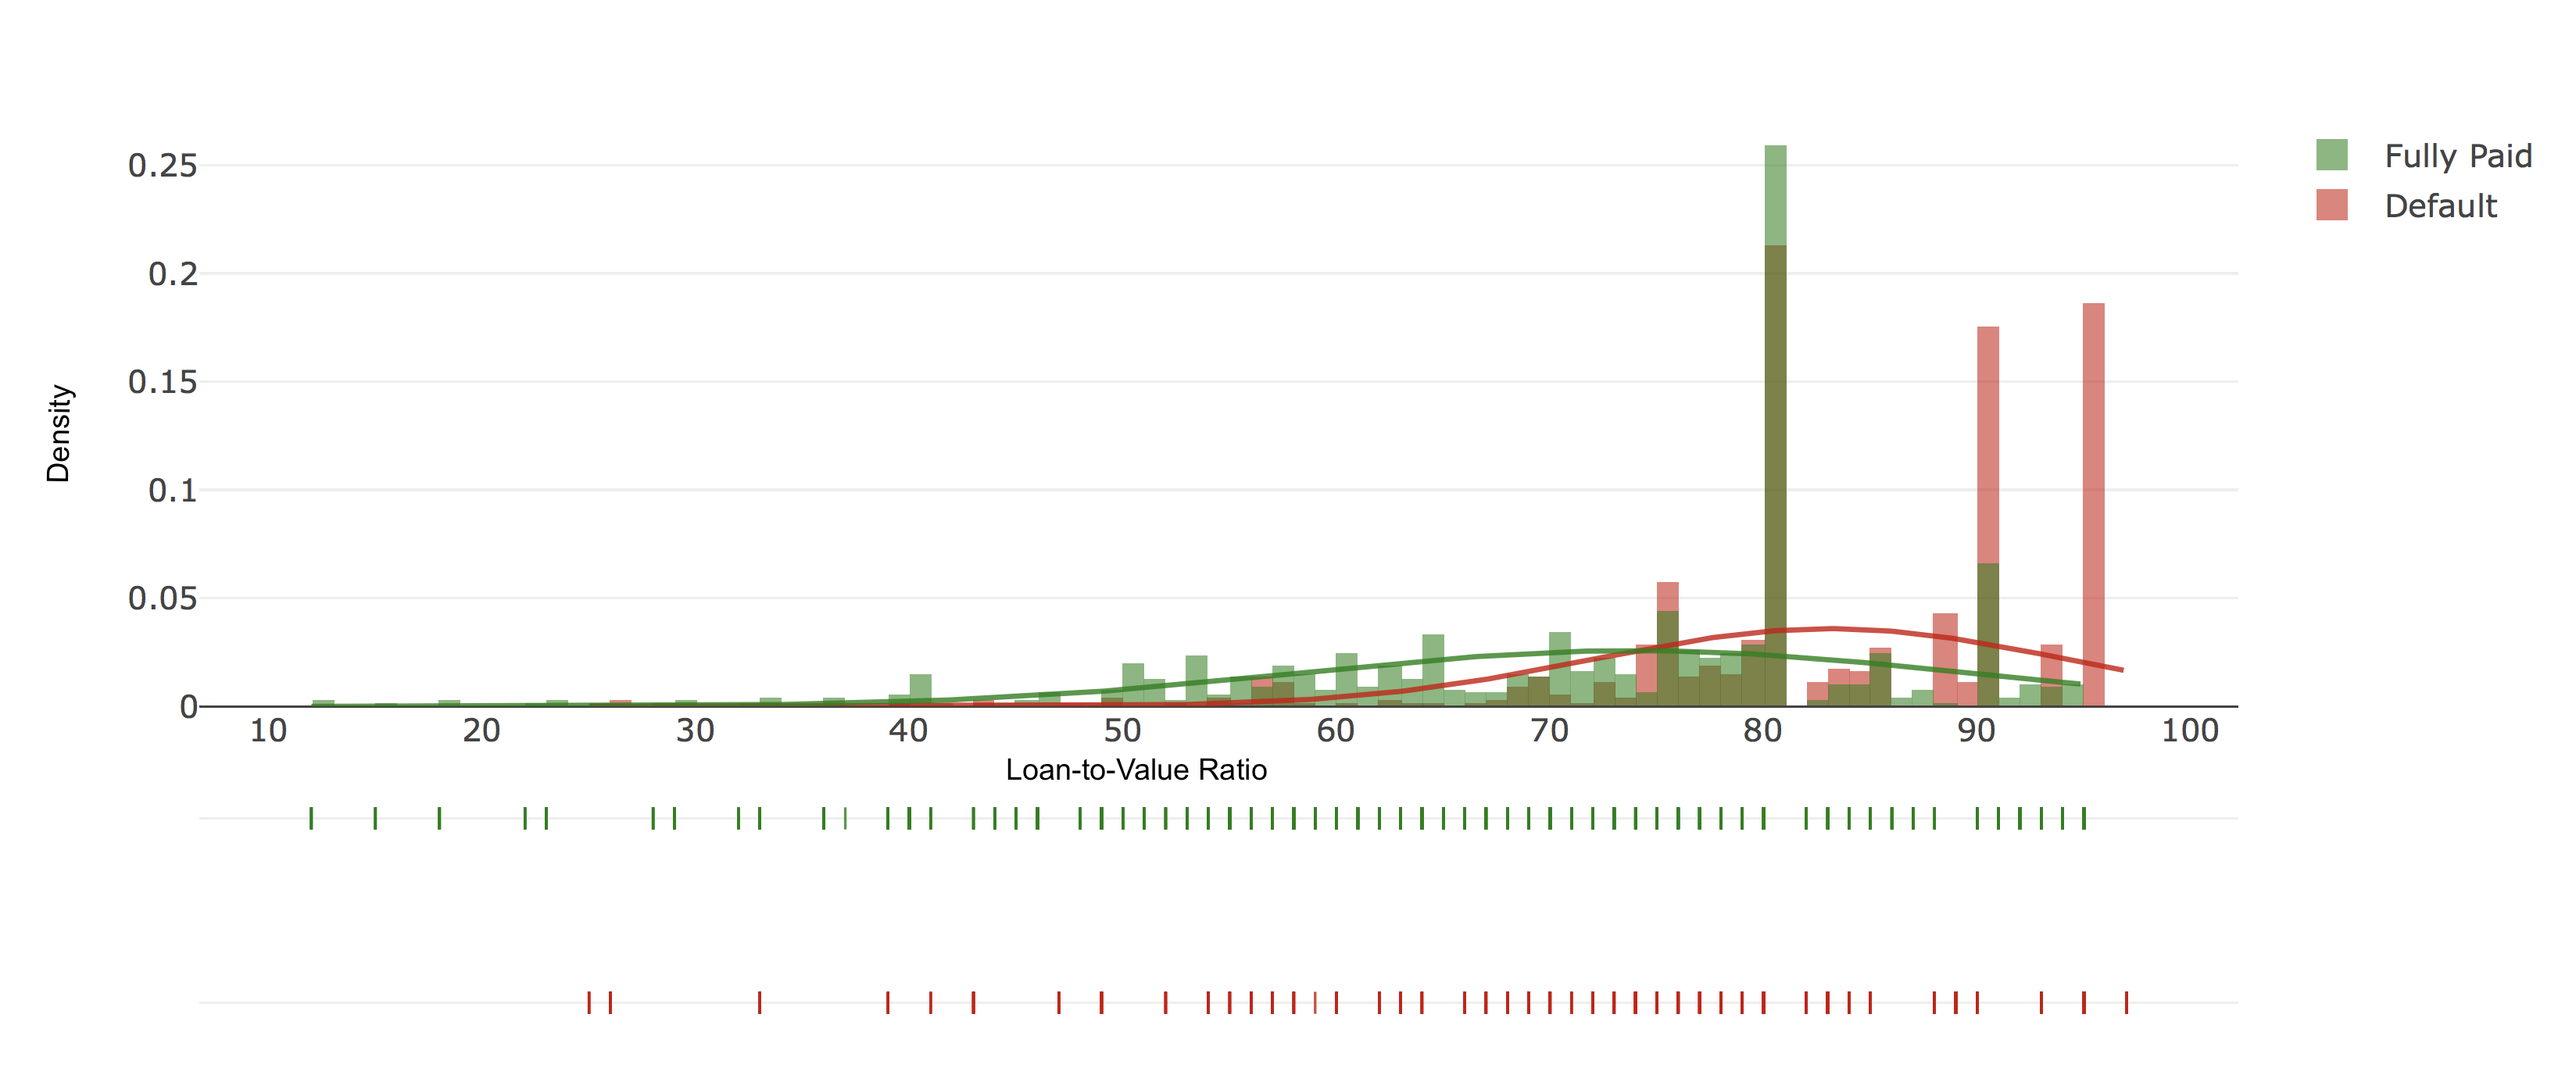
\includegraphics[width=1.1\textwidth]{Images/ltv_dist.png}
                \caption{Density Plot with Normal Distribution and Rug plot - A comparison between Fully Paid and Default loans using the feature Loan-to-Value Ratio}
                \label{fig:ltv}
            \end{figure}
            
            We observed that in both figure \ref{fig:ltv} and figure \ref{fig:FICO_score} there was a moderate level of separability. The normal distribution curves for 'Fully Paid' and Default' overlap significantly on both graphs; this shows that the data is not linearly separable using only these features. This is confirmed by the distribution of the rug plots which show that the spread of data is large across the two categories ('Fully Paid' and 'Default') on both graphs. This observation suggests that the machine learning methods (such as neural networks) should out-perform linear regression models, as they are able to find non-linear relationships in the origination features to perform the classification task. 
    
        \subsection{Performance Features} \label{monthly_update_features}
            As mentioned in Section \ref{data_cleaning}, many of the features defined in the performance updates are only relevant at the end of the mortgage. We, therefore, removed these features from the performance vector. However, the frequency and completeness of the performance updates that are relevant allowed us to create new features. Specifically, we captured historical trends for each loan, obtained from performance updates that preceded the current month. For example, we calculated the number of times a particular loan had been 30 days delinquent. 
            
            Previous work has validated the predictive performance of these indicators; \citeauthor{default_risk_2005} showed that loans with more frequent delinquency periods, when combined with higher FICO (Credit) scores, were less likely to foreclosure. The method we used to track delinquency periods is as follows. We calculated the occurrence of each $\textbf{Status}$\footnotemark[\getrefnumber{footnote_status}] for a particular loan, by iterating over all previous performance updates for that loan. This produces multiple features per loan that act as status counters, i.e. every time a particular loan enters a state, the counter will be incremented. 
            
            
            Additionally, the work by \cite{default_risk_2011} and \cite{mortgage_risk} found that using indicators that capture short-term trends are beneficial when predicting foreclosure rate. We therefore created another set of features which only considered the occurrence of each $\textbf{Status}$\footnotemark[\getrefnumber{footnote_status}] over the last 12-months. 
            
            A full list of the performance update features can be seen in table \ref{4: Monthly_update_features}. 

            
            \stepcounter{footnote}\footnotetext{The status of a loan is defined in this work as either current, 30, 60, 90+ days delinquent, Foreclosed, REO (Real-Estate Owned) or Fully Paid. \label{footnote_status}}
            
            \begin{center}
                \begin{table}[H]
                    \centering
                    \begin{tabular}{|p{11.5cm}|p{2.5cm}|}
                        \hline \textbf{Loan Feature} & \textbf{Values} \\ \hline \hline
                        Current Status & $\textbf{Status}$ \\ \hline  
                        Current Unpaid Principal Balance & Continuous \\ \hline  
                        Current Interest Rate & Continuous \\ \hline  
                        Loan Age & Continuous \\ \hline  
                        Months Remaining & Continuous \\ \hline  
                        Percentage change between Last Balance \& Current Balance & Continuous \\ \hline   
                        Occurrences of $\textbf{Status}$ \footnotemark[\getrefnumber{footnote_source_1}] & Continuous \\ \hline
                        Occurrences of $\textbf{Status}$ in the last 12 months \footnotemark[\getrefnumber{footnote_source_1}] & 0-12 \\ \hline
                        Interest Rate -− National Interest Mortgage Rate \footnotemark[\getrefnumber{footnote_source_1}] & Continuous \\ \hline
                        Number of Months that Mortgage Interest Rate $<$ National Interest Rate \footnotemark[\getrefnumber{footnote_source_1}] & Continuous \\ \hline 
                    \end{tabular}
                    
                    \vspace*{0.2cm}
                
                    {\footnotesize $\textbf{Status}$ = \{Current, 30, 60, 90+ Days Delinquent, Foreclosed\footnotemark[\getrefnumber{footnote_default}], REO or Fully Paid,\}}
                
                    \caption{Performance Features} \vspace{0.5cm}
                    \label{4: Monthly_update_features}
                \end{table}
            
                \stepcounter{footnote}\footnotetext{Feature concept taken from \cite{mortgage_risk} \label{footnote_source_1}}
                
            \end{center}
            
            % \unsure[inline]{CHECK THAT THE FOOTNOTE IN TABLE IS ON SAME PAGE £((@)£!@@@!}

            For clarity, we explain a subset of features from table \ref{4: Monthly_update_features} using a language description:
            
            \begin{itemize}
              \item \textbf{Occurrences of 30-dd} represents the number of times the current loan has entered the 30 days delinquent status up to the current time. 
              \item \textbf{Occurrences of 30-dd in the last 12 months} represents the number of times the current loan has entered the 30 days delinquent status in the last 12 months. 
            \end{itemize}
            
            \clearpage
            
            \subsubsection{Evaluation of 12-month performance indicator}
            
            Figure \ref{fig:30dd} and \ref{fig:30dd_12months} show the comparison between Fully Paid and Default loans using the feature 'Occurrences of 30-dd' and 'Occurrences of 30-dd in the last 12 months' respectively. The chart in \ref{fig:30dd} shows that there are more Fully Paid than Default loans that have fewer occurrences of 30-day delinquency when considering the full lifetime of a loan. 
            
            
            
            \begin{figure}[H]
                \centering
                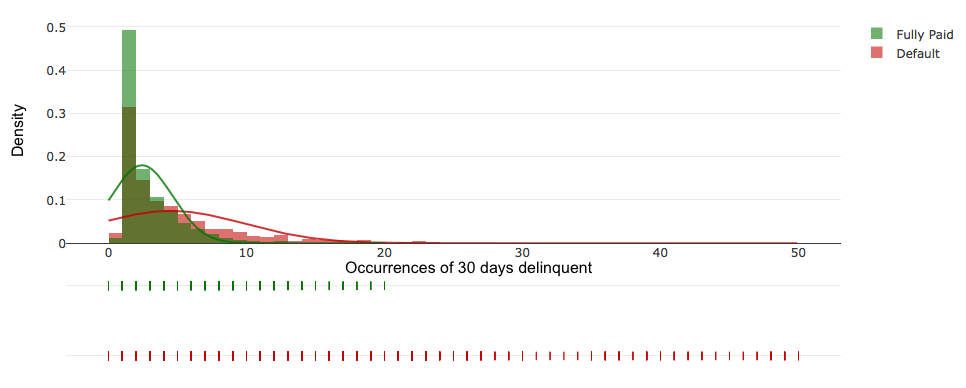
\includegraphics[width=0.99\textwidth]{Images/occur_30_dd_dist.png}
                \caption{A comparison between Fully Paid and Default loans using the feature 'Occurrences of 30-dd'.}
                \label{fig:30dd}
            \end{figure}
            
            \begin{figure}[H]
                \centering
                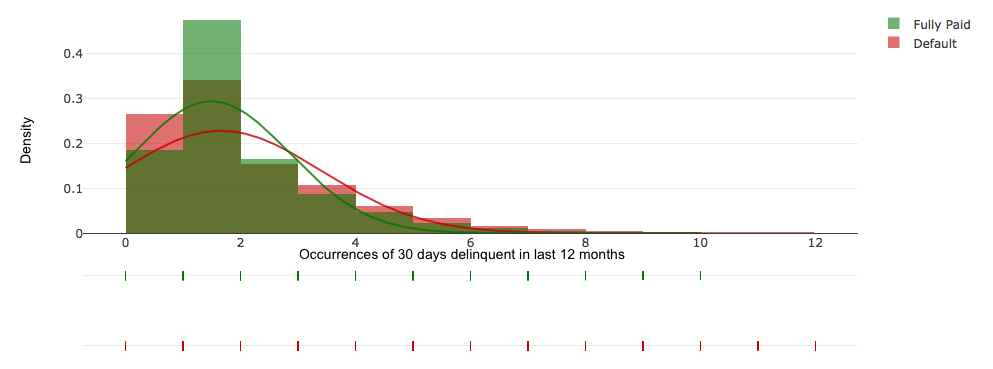
\includegraphics[width=0.99\textwidth]{Images/occur_30_dd_12_mon_dist.png}
                \caption{A comparison between Fully Paid and Default loans using the feature 'Occurrences of 30-dd in the last 12 months'.}
                \label{fig:30dd_12months}
            \end{figure}
            
            If we compare figure \ref{fig:30dd} and \ref{fig:30dd_12months}, we find that the relationship is less apparent in \ref{fig:30dd_12months}. This suggests that loan performance indicators which are based on only recent loan history, i.e. the last 12 months, are less powerful and relevant to the prediction. Nevertheless, we use both types of indicators as features in our data as there may exist non-linear relationships that are more difficult to identify. 
            


        
        
        \subsection{Economic Features} \label{economic_update_features}
            The magnitude of the dataset allows us to obtain novel features based on location (per State and per Zipcode). A full list of the Economic features can be seen in table \ref{4: table_economic_performance_features}.
            
             \begin{table}[H]
                \centering
                \caption{Economic Performance Features} \vspace{0.5cm}
                \label{4: table_economic_performance_features}
                \begin{tabular}{|p{11.5cm}|p{2.5cm}|}
                    \hline \textbf{Loan Feature} & \textbf{Values} \\ \hline \hline
    
                    Monthly National Mortgage Interest Rate \footnotemark[\getrefnumber{footnote_mr12}] & Continuous \\ \hline
                    
                    Monthly Housing Price Index per State & Continuous \\ \hline
                    Monthly Unemployment Rate per State \footnotemark[\getrefnumber{footnote_mr12}] & Continuous \\ \hline
                    
                    Number of Loans (active) per State & Continuous \\ \hline
                    Number of Loans (active) per Zipcode & Continuous \\ \hline
                    
                    Number of Loans (taken out) per State & Continuous \\ \hline
                    Number of Loans (taken out) per Zipcode \footnotemark[\getrefnumber{footnote_mr12}] & Continuous \\ \hline
                    
                    Number of Loans (taken out) per State in the last 12 months & 1-12 \\ \hline
                    Number of Loans (taken out) per Zipcode in the last 12 months & 1-12  \\ \hline
                
                    Default Rate per State & Continuous \\ \hline
                    Default Rate per Zipcode & Continuous \\ \hline
                    
                    Default Rate per State in the last 12 months & Continuous \\ \hline
                    Default Rate per Zipcode in the last 12 months \footnotemark[\getrefnumber{footnote_mr12}] & Continuous \\ \hline
                    
                    Occurrences of Paid Off \& Default per State & Continuous \\ \hline
                    Occurrences of Paid Off \& Default per Zipcode & Continuous \\ \hline
                    
                    Occurrences of Paid Off \& Default per State in the last 12 months & 1-12  \\ \hline
                    Occurrences of Paid Off \& Default per Zipcode in the last 12 months & 1-12  \\ \hline
                    
                \end{tabular}
                
            \end{table}
            \stepcounter{footnote}\footnotetext{ Feature concept taken from \cite{mortgage_risk} \label{footnote_mr12}}
            
            % \unsure[inline]{CHECK THAT THE FOOTNOTE IN TABLE IS ON SAME PAGE £((@)£!@@@!}
            
            As discussed in section \ref{related_work}, the work by \cite{default_risk_2011} and \cite{mortgage_risk} found that using indicators that capture short-term economic trends are beneficial when predicting foreclosure rate. They also found an association with neighbouring characteristics and higher default rates. Building on these findings, we produced several location-based features that capture both short and long-term trends. We were able to calculate the total number of loans, total number of Paid Off loans, and total number of Default loans, on a per state and zip code basis across each month (the complexity of this is discussed in Section \ref{manipulation}). Using this data, we calculated the Default rate on a per state and zip code basis across each month. We also created an additional feature set which only considered the last 12 months of history, similar to section \ref{monthly_update_features}.
            
            For clarity, we explain a subset of features from table \ref{4: table_economic_performance_features} using a language description:
            
            \begin{itemize}
              \item \textbf{Occurrences of Default per State} represents the number of loans that have Defaulted in the same state as the current loan up to the current time. 
              \item \textbf{Occurrences of Paid Off per Zipcode in the last 12 months} represents the number of loans that have Fully Paid in the same zipcode as the current loan over the last 12 months.
            \end{itemize}
            
            From figure \ref{fig:default_per_st} and \ref{fig:default_per_st_12_months}, we observe higher levels of separability between 'Default' and 'Fully Paid' when comparing the distribution on feature 'Occurrences of Default per State in the last 12 months' (figure \ref{fig:default_per_st_12_months}) to 'Occurrences of Default per State' (figure \ref{fig:default_per_st}). The graph that considers only the last 12 months indicates that the majority of Fully Paid loans occur in states where the Occurrence of Default is lower. We concluded that geographically based features which consider only recent history, i.e. the last 12 months, can be more powerful and relevant to the prediction than features that capture the entire historical period (from 1999 up to the current time of the loan). This difers from our findings in section \ref{monthly_update_features} where we state that loan performance indicators which consider only recent history, i.e. the last 12 months, seems to be less powerful when compared to looking at the entire duration of the loan. 
            
            \begin{figure}[H]
                \centering
                \hspace*{-0.5cm}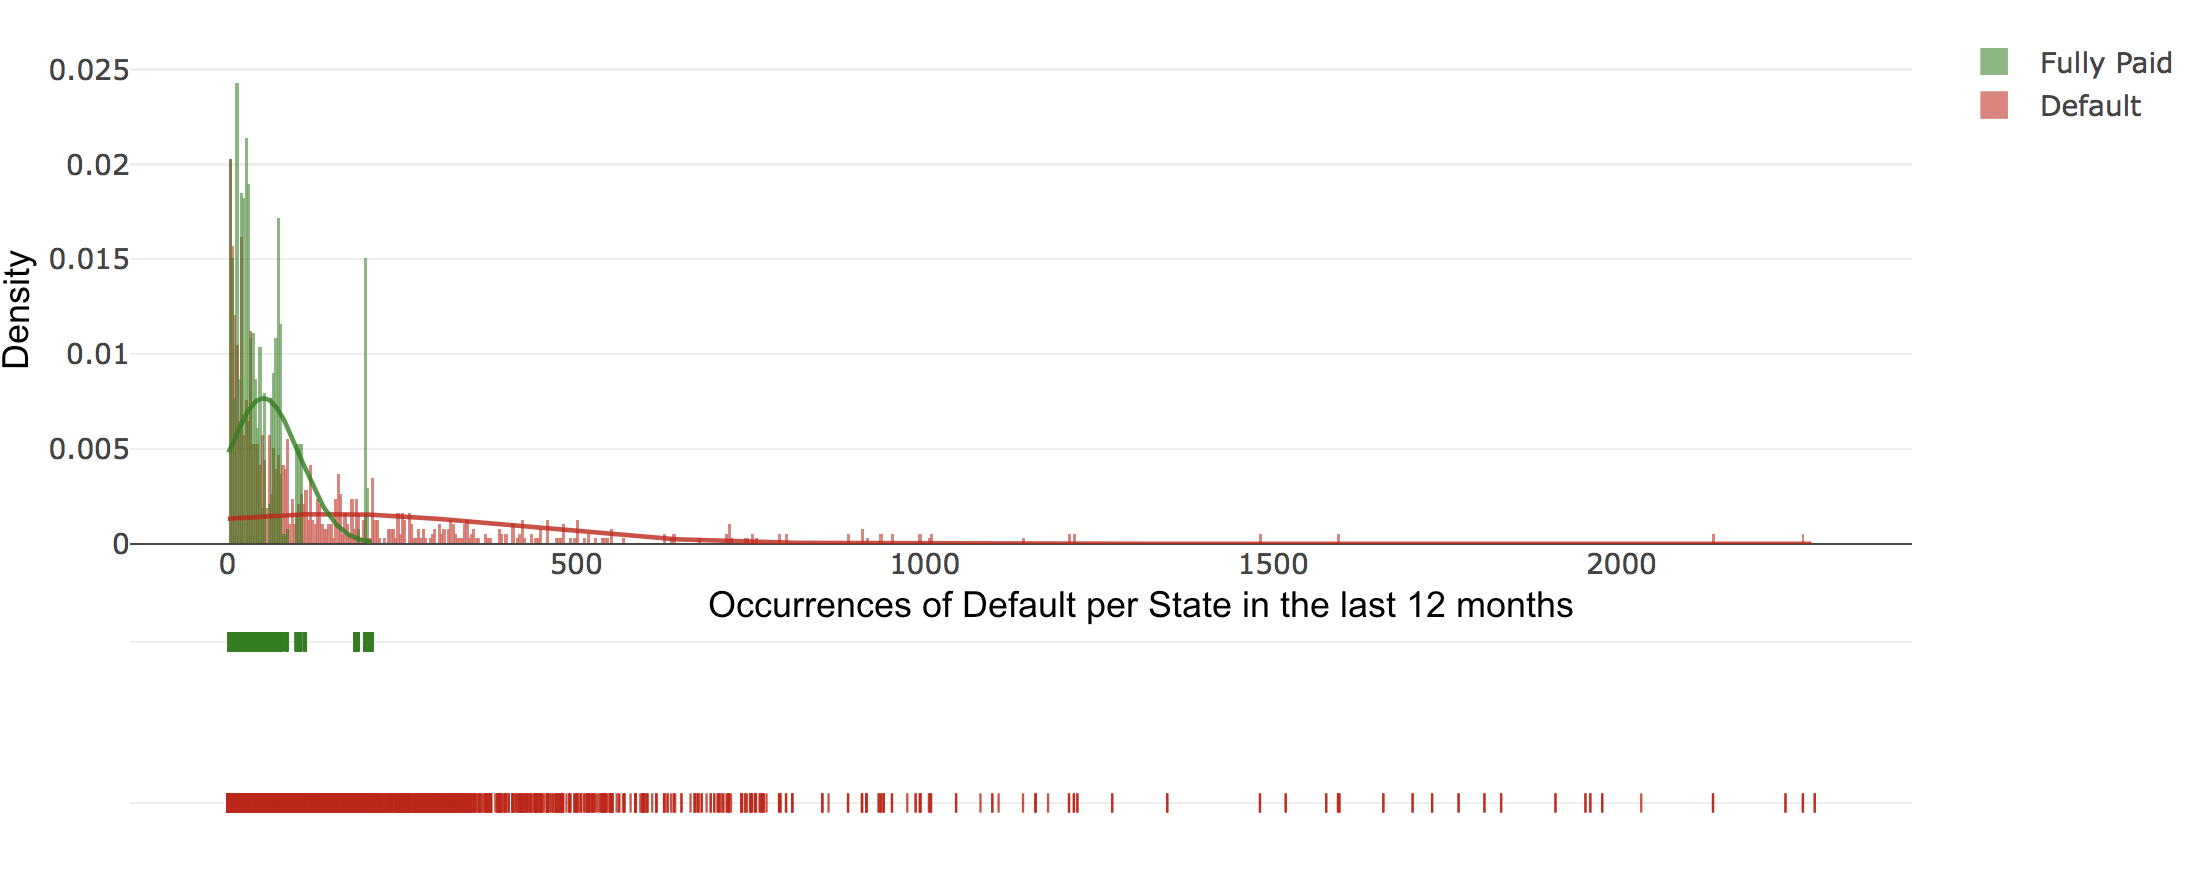
\includegraphics[width=1.1\textwidth]{Images/occr_default_per_state_12_mon_12_mon.png}
                \caption{Density Plot with Normal Distribution and Rug plot - A comparison between Fully Paid and Default loans using the feature 'Occurrences of Default per State in the last 12 months'}
                \label{fig:default_per_st_12_months}
            \end{figure}
            
            \begin{figure}[H]
                \centering
                \hspace*{-0.5cm}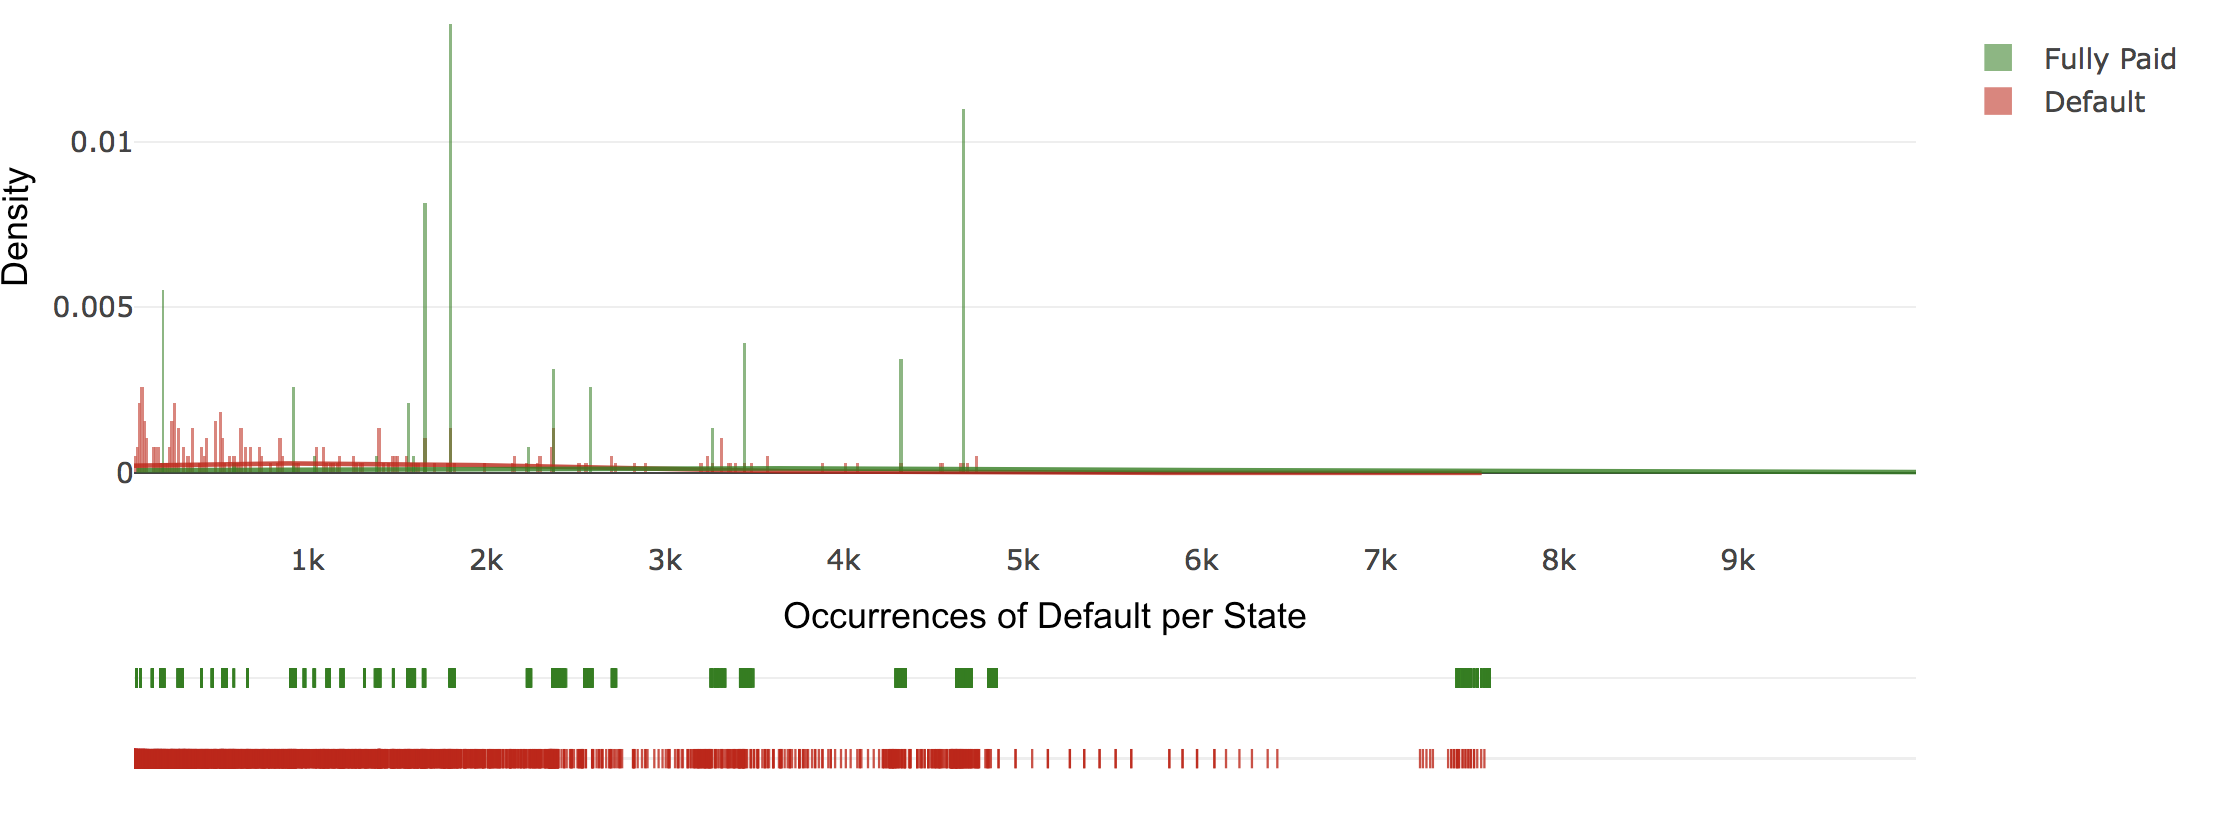
\includegraphics[width=1.1\textwidth]{Images/occr_default_per_state_dist.png}
                \caption{Density Plot with Normal Distribution and Rug plot - A comparison between Fully Paid and Default loans using the feature 'Occurrences of Default per State'}
                \label{fig:default_per_st}
            \end{figure}

            Additionally, the work by \cite{default_risk_2011} and \cite{mortgage_risk} showed a correlation between economic information such as housing market conditions and the rate of foreclosure.  We, therefore, introduced three new datasets; Monthly Housing Price Index per State, Monthly Unemployment Rate per State, and National Monthly Interests rates, all acquired from the \citeauthor{labor_stats} [\citenum{labor_stats}]. A comparison of the feature Housing Price Index can be seen in figure \ref{fig:housing_price_index}, where we observe significant levels of separability between 'Default' and 'Fully Paid'. We, therefore, concluded that we find a correlation between Housing Price Index and the occurrence of a default. 
                
            \begin{figure}[H]
                \centering
                \hspace*{-0.5cm}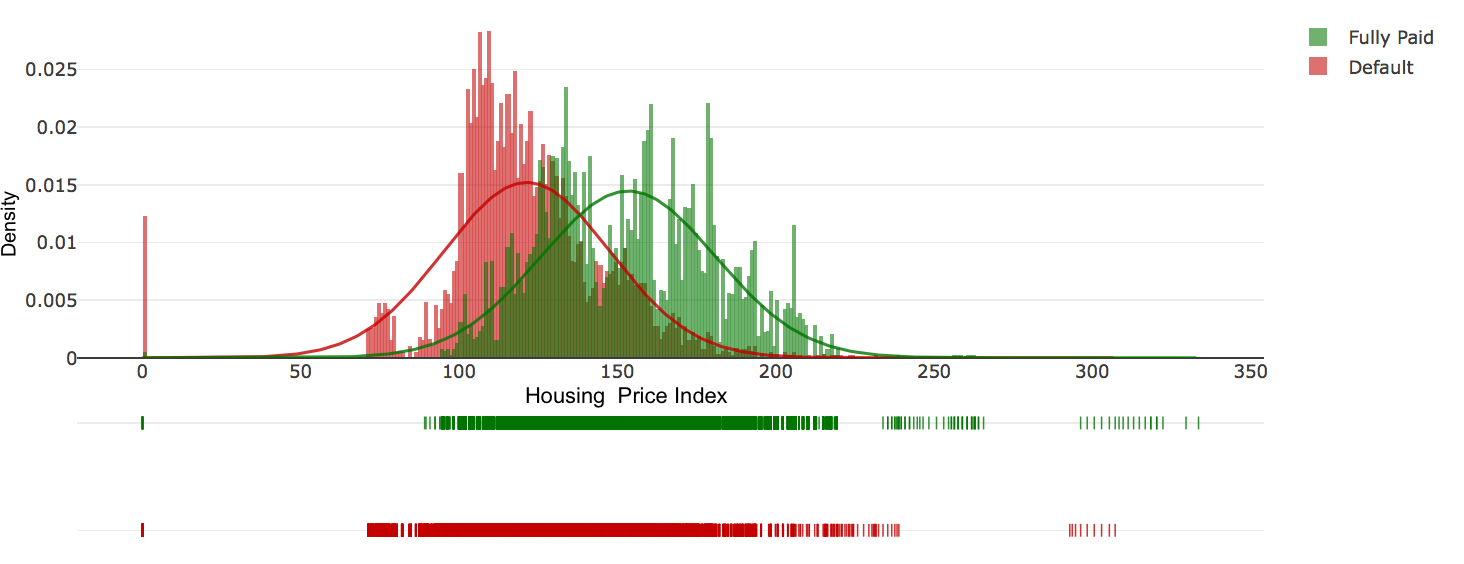
\includegraphics[width=1.1\textwidth]{Images/housing_price_index_dist.png}
                \caption{Density Plot with Normal Distribution and Rug plot - A comparison between Fully Paid and Default loans using the feature Housing Price Index}
                \label{fig:housing_price_index}
            \end{figure}
                
        
        
        
    
    \clearpage
    
    \section{Data Processing}
        The dataset in its raw form was over 150GBs. As a consequence, we required significant computation processing capacity in order to manipulate the data and train the model. We used the University of Bristol's Super-Computer, Blue Crystal 4, utilising the Computational Processing Units (CPUs) for data manipulation as discussed in Section \ref{manipulation}, and the Graphical Processing Units (GPUs) for training the model as discussed in Section \ref{loading}. To access Blue Crystal 4, we were required to log-in remotely to a Linux Server using Secure Shell (SSH\footnote{The SSH protocol is a method for secure remote login from one computer to another}). This provided access to a 'login' node from which we could submit code to be run on the CPUs and GPUs, using an open-source cluster management and job scheduling system called Slurm. 
        
        
        \subsection{Implementation}
            We chose to use the programming language Python for the implementation of this work. Python has numerous well documented libraries for large-scale data manipulation, namely \citeauthor{numpy} [\citenum{numpy}] and \citeauthor{pandas} [\citenum{pandas}], as well as a comprehensive library for building and training neural networks, namely \citeauthor{tensorflow} [\citenum{tensorflow}]. The use of these libraries meant that it was not necessary to implement the low-level code needed to train a neural network, saving time and eliminating unnecessary complexity. The information in table \ref{python_libraries} gives an overview of the main Python libraries that were used in this work.
           
            \begin{table}[H]
                \centering
                \caption{Overview of Python Libraries and Use-Cases} \vspace{0.5cm}
                \label{python_libraries}
                \begin{tabular}{|p{4cm}|p{1.75cm}|p{7.25cm}|}
                    \hline \textbf{Python Library} & \textbf{Version} & \textbf{Use-Case} \\ \hline \hline
                    
                    \citeauthor{tensorflow} [\citenum{tensorflow}] & 1.2 & Training neural network. \\ \hline
                    \citeauthor{tensorboard} [\citenum{tensorboard}] & 1.6.0 & Visualisation of training \& results of neural network \\ \hline
                    \citeauthor{cuda} [\citenum{cuda}] & 8.0 & Interface with Nvidia GPU \\ \hline
                    \citeauthor{pandas} [\citenum{pandas}] & 0.22.0 & Data manipulation \\ \hline
                    \citeauthor{numpy} [\citenum{numpy}] & 1.14.1 & Data manipulation \\ \hline
                    \citeauthor{multitasking} [\citenum{multitasking}] & 0.0.7 & Asynchronous loading \\ \hline
                
                \end{tabular}
            \end{table}

        \subsection{Loading} \label{loading}
            The dataset was split over multiple CSV (Comma Separated Values) files. For each year, the data was split into four quarters, each containing two files. To manipulate the data we used Pandas Data Frames in Python. In order to speed up the file I/O (Input/Output), we used the HDF5 \footnote{a file format designed to store and organise large datasets in hierarchical structures} file format with the main benefit being the application of data chunking. This meant that the data could be stored in a non-continuous block of memory, which allowed us to read/write Pandas Data Frames directly to secondary memory much more efficiently. In the worst case, this reduced the load time for one file from 35s to 11s, and in the best case from 169s to 39s. When applied to all files, this provided significant speed benefits. One drawback to using the HDF5 file format is that the files sizes increase significantly and required, on average, five times more space to store the same data. 
            
            Nevertheless, the speed improvement was especially useful when training the neural network as it contributed to the seamless transition between batches across multiple files. To achieve this transition, we created an asynchronous loading pattern. The pattern works as follows: We load and process the current file, the network begins training on the new data, at which point we asynchronously requested the next file and processed the data ready for the network. This processing technique allowed us to perform manipulation such as data resampling before the neural network has finished iterating over the previous data. Although it would have been possible to resample the entire dataset before training, by writing the resampled data to file, the asynchronous approach allowed for a much faster and friction-less workflow. Note that, for training and testing the models, we used a Nvidia Pascal P100 GPU.

        \subsection{Manipulation} \label{manipulation}
            Performing operations on data of this scale turned out to be very challenging. The main issue was that to perform operations on the data in any reasonable amount of time; it was necessary to use group-wise operations using functions from Python Pandas Library. This restriction meant that the task of calculating the cumulative totals, i.e. the number of defaulted loans per state, as mentioned in Section \ref{economic_update_features}, across the entire dataset was especially challenging. 
            
            To process the data, we initially used a 14 core 2.4 GHz Intel E5-2680 v4 (Broadwell) CPU with 128 GiB of RAM. However, we encountered some memory issues when manipulating the dataset. A python 'MemoryError' was the most common, indicating that the virtual address space limit was reached. This issue subsided after switching the same CPU chip with 512 GiB of RAM. To perform the operations mentioned in Section \ref{sec: Feature_Engineering} took 5 days. Further, we used only single precision floating point values, and although this does not affect the output of the model, it approximately halves the memory requirement which resulted in a computational speed up.
            
        
        \subsection{Model Preparation}
            We used a one hot encoding format to represent all categorical data. This format allowed categorical variables to be represented using binary vectors. For example, the feature 'st' is the state category where each state is represented using a two-letter string ('NY', 'WT'... etc.). In this case, we created a new feature for each state ('st\_NY', 'st\_WT'... etc.), where either a 1 or 0 is used to represent the presence of that state. 
            
            It is important to randomly shuffle the data before passing the information to the model. We used a native Python random shuffle function, using a date-stamp (HH + MM + SS), as the random seed. Although not cryptography secure, this source of randomness is simple, quick and frequently changes, which is more than suitable for the intended purpose.
            

    \clearpage

    \section{Formal Description} \label{formal_description}
        We use three vectors to construct the dataset for the final model, the origination vector (appendix \ref{appendix: table_american_loan_features_origination}), performance vector (table \ref{4: Monthly_update_features}), and economic performance vector (table \ref{4: table_economic_performance_features}). The following description is used to formalise the structure of the data.
        
        \vspace{0.5cm}
        
        \noindent We adopt a discrete time interval for the periods $t = 0,1,2, ..., months$. We define:
        \begin{itemize}
          \item $\textbf{O}$ to be the Origination vector of length p; 
          \item $\textbf{M} (t)$ to be the Performance vector, at time t, of length q;
          \item $\textbf{E} (t)$ to be the Economic performance vector, at time t, of length r;
        \end{itemize}
        $i.e.$
        \begin{equation}
            \textbf{O} = \begin{bmatrix}
                   O _0 \\[0.3em]
                   O_1 \\[0.3em]
                   \vdots \\[0.3em]
                   O _p
                 \end{bmatrix}
            \quad \textrm{,} \quad
            \textbf{M} (t) = \begin{bmatrix}
                   O _0 (t) \\[0.3em]
                   O_1 (t) \\[0.3em]
                   \vdots \\[0.3em]
                   O _q (t)
                 \end{bmatrix}
            \quad \textrm{and, } \quad
            \textbf{E} (t) = \begin{bmatrix}
                   E _0 (t) \\[0.3em]
                   E_1 (t) \\[0.3em]
                   \vdots \\[0.3em]
                   E _r (t)
                 \end{bmatrix}
            \quad \textrm{.}
        \end{equation}
        
        \vspace{20pt}
        
        \noindent Let $\textbf{X}(t)$ be a vector of length $p + q + r + 3$ consisting of elements $X _i (t)$ for $i\: \epsilon\: \{0,1,..., p + q + r + 2\} $, and
        
        \vspace{20pt}
        
        \begin{adjustwidth}{2.5em}{0pt}
            where:
            \begin{equation}
                X _i (t) = 
                    \begin{cases}
                        O _i      & \forall \qquad  i\: \epsilon\: [0, p], \\
                        M _{i - (p + 1)}\: (t)  & \forall \qquad  i\: \epsilon\: [p + 1, p + q + 1], \\
                        E _{i - (p + q + 2)}\: (t)  & \forall \qquad  i\: \epsilon\: [p + q + 2, p + q + r + 2]. \\
                    \end{cases}
           \end{equation} 

           \vspace{20pt}

        \end{adjustwidth}
       
        \noindent Define X be the matrix formed by the columns $(\textbf{X} (0),\: \textbf{X} (1),\: ...)$.

            
        \vspace{20pt}



    \subsubsection{Conclusion}
        In this chapter, we introduced the Freddie Mac Single-Family dataset and the methods by which we used to process, load and prepare the data for training the model. We discussed our approach when creating new features based on geography and loan performance information from within the dataset. As well as introducing additional economic data, which included Housing Price Index, Unemployment rates, and National Interests rates. We then introduced the same set of features but which only consider the recent past, i.e. the last 12 months. We found that these indicators are more effective when applied to economic and geographical based features and less so when applied to individual loan performance features. 
        
        
        
        